Cloud Firestore es el servicio de base de datos de Google Firebase para aplicaciones móviles. Firestore permite una experiencia de programación increíble cuando se usa en un stack de aplicaciónes completo. Los datos en tiempo real y la facilidad de conexión a la base de datos hacen que FERN Stack sea una forma rápida de conectar estas tecnologías.
\vspace{0.8cm}

Firestore es una base de datos orientada a documentos, toda la información se guarda en colecciones como en un JSON, principalmente diseñada para almacenar, recuperar y administrar información orientada a documentos, también conocida como datos semiestructurados. La \gls{escalabilidad} es completamente automática, lo que significa que no es necesario compartir sus datos en varias instancias. Los cargos de Cloud Firestore se basan en las operaciones realizadas en su base de datos (lectura, escritura, borrado), ancho de banda y almacenamiento. Admite límites de gasto diario para proyectos de Google App Engine, para garantizar que no exceda los costos con los que el usuario se sienta cómodo.
\vspace{0.8cm}

\begin{figure}[H]
  \centering
  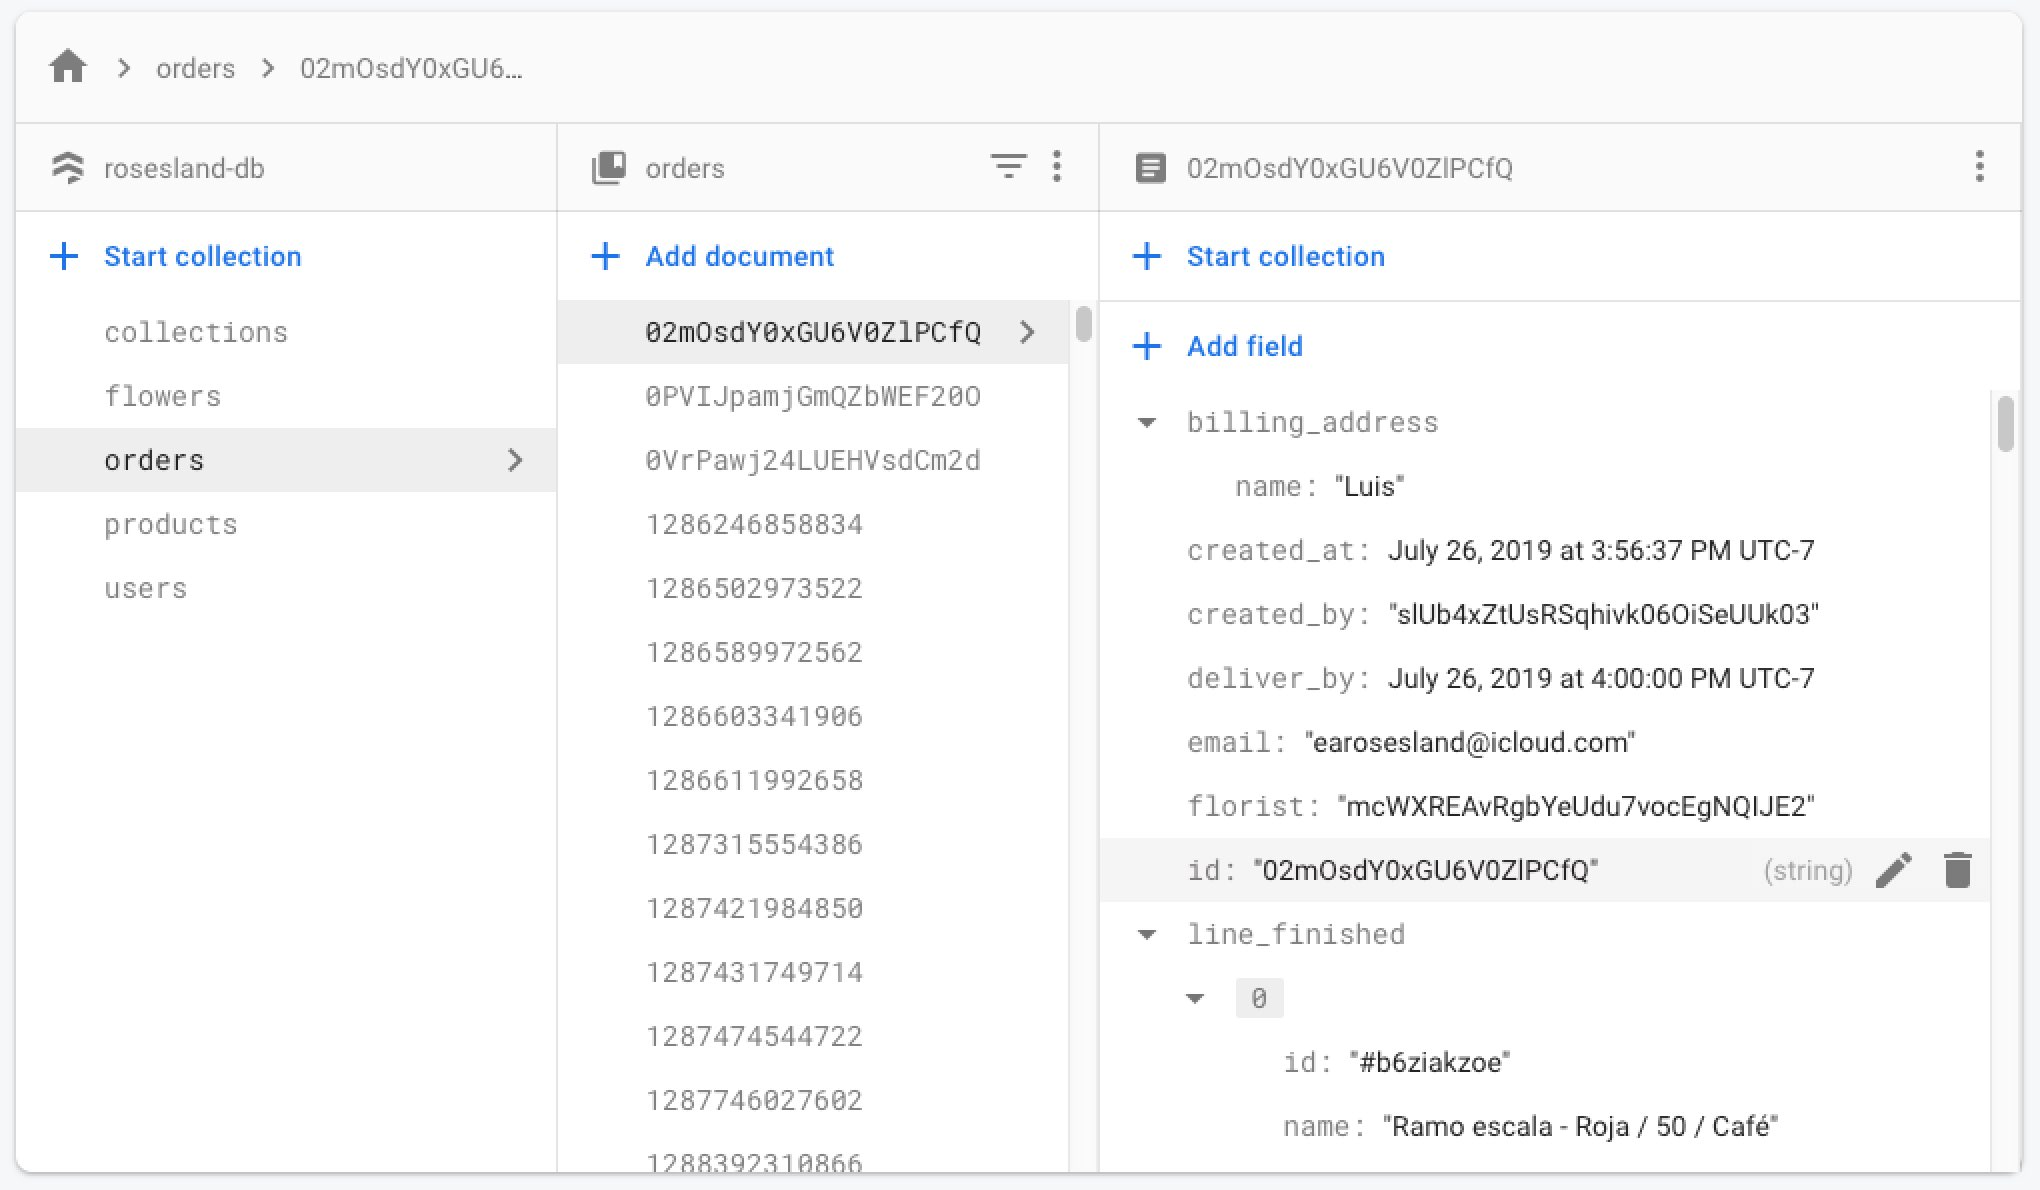
\includegraphics[width=0.9\textwidth]{firestore}
  \caption{Colección de Firestore con sus documentos internos. (Fuente: Elaboración propia)}
\end{figure}